%%%%%%%%%%%%%%%%%%%%%%%%%%%%%%%%%%%%%%%%%
% Thin Sectioned Essay
% LaTeX Template
% Version 1.0 (3/8/13)
%
% This template has been downloaded from:
% http://www.LaTeXTemplates.com
%
% Original Author:
% Nicolas Diaz (nsdiaz@uc.cl) with extensive modifications by:
% Vel (vel@latextemplates.com)
%
% License:
% CC BY-NC-SA 3.0 (http://creativecommons.org/licenses/by-nc-sa/3.0/)
%
%%%%%%%%%%%%%%%%%%%%%%%%%%%%%%%%%%%%%%%%%

%----------------------------------------------------------------------------------------
%	PACKAGES AND OTHER DOCUMENT CONFIGURATIONS
%----------------------------------------------------------------------------------------

\documentclass[a4paper, 12pt]{article} % Font size (can be 10pt, 11pt or 12pt) and paper size (remove a4paper for US letter paper)

\usepackage[protrusion=true,expansion=true]{microtype} % Better typography
\usepackage[frenchb]{babel}
\usepackage{graphicx} % Required for including pictures
\usepackage{wrapfig} % Allows in-line images

\usepackage{mathpazo} % Use the Palatino font
\usepackage[utf8]{inputenc} % UTF-8 encoding for input, to get french special characters recognized
\usepackage[T1]{fontenc} % Required for accented characters
\linespread{1.05} % Change line spacing here, Palatino benefits from a slight increase by default
\usepackage{parskip} % add some space between paragraph 
 
\makeatletter
\renewcommand\@biblabel[1]{\textbf{#1.}} % Change the square brackets for each bibliography item from '[1]' to '1.'
\renewcommand{\@listI}{\itemsep=0pt} % Reduce the space between items in the itemize and enumerate environments and the bibliography

\renewcommand{\maketitle}{ % Customize the title - do not edit title and author name here, see the TITLE block below
\begin{flushright} % Right align
{\LARGE\@title} % Increase the font size of the title

\vspace{50pt} % Some vertical space between the title and author name

\vspace{40pt} % Some vertical space between the author block and abstract
\end{flushright}
}

\begin{document}

%----------------------------------------------------------------------------------------
%	ESSAY BODY
%----------------------------------------------------------------------------------------

\tableofcontents
\newpage
\section{Avant-propos}
\subsection{Remerciements}
Nous tenons à remercier :

M. Alain LIORET, notre maître de mémoire, pour son soutien, sa passion, et pour nous avoir guidé dans notre travail. Il nous a donné de très bonnes pistes de recherches, ainsi que de bons conseils dans nos choix.

L’équipe pédagogique de l’ESGI, pour la qualité des cours dispensés à l’ESGI, qui nous ont donné la motivation nécessaire pour rédiger ce mémoire.

\newpage
\subsection{Résumé}
Les jeux vidéo sont de plus en plus beaux, que ce soit en approchant le photoréalisme, ou en ayant une patte graphique unique. Ils sont également de plus en plus profonds, avec une histoire, une narration et un univers toujours plus poussés. Le gameplay également n’a de cesse de s’améliorer, que ce soit à travers de nouvelles idées innovantes de game design, ou via de nouveaux périphériques pour renforcer l’interaction ainsi que l’immersion du joueur. 

Mais le domaine dans lequel il reste le plus de progrès à faire pour proposer des expériences toujours plus intéressantes et immersives est l’intelligence artificielle (IA). Bien que celle-ci soit de plus en plus présente (et attendue) dans les jeux, et de plus en plus évoluée grâce à des algorithmes toujours plus performants, cela reste en général une IA « fixe », avec des comportements prévus à l’avance, en réponse à des évènements prévus à l’avance.

En effet, bien souvent les personnages non joueurs (PNJ) sont des entités statiques du jeu ne possédant qu’un panel fixe d’actions ou de répliques de dialogues, qu’ils soient alliés (marchand), ou ennemis (monstre). Ces personnages sont ainsi relégués au rang d’élément du décor, alors qu’ils pourraient occuper une place bien plus importante dans le jeu, apportant à la fois en profondeur de gameplay et de narration.

Dans ce mémoire, nous étudierons les différentes IA qui existent actuellement, ainsi que ce qu’elles apportent en termes d'expérience.

\newpage
\subsection{Abstract}
Video games are more and more beautiful, whether it be by approaching photorealism, or by using a unique graphic style. They’re also more and more deep, with a story, a narration and an universe always more advanced. The gameplay keeps getting better, either with innovative game design ideas, or with new devices to enhance the interaction and immersion of the player.
 
But there is a field in which much progresses are yet to be done in order to offer ever more interesting and immersive experiences, and this field is artificial intelligence (AI). Although it’s more and more present (and expected) in video games, and more and more efficient through algorithms ever more powerful, it remains, in general a scripted AI, with programmed behaviors which respond to specific events. 

Indeed, often the non-player characters (NPCs) are static entities of the game with only a fixed panel of actions or dialogues replicas, whether allies (merchant) or enemies (monster). These characters are relegated to the role of decorative elements, when they could take a more important place in the game, providing both depth of gameplay and storytelling.
In this thesis, we will study the state of the art of artificial intelligence applied on NPCs, and what they offer in term of experience.

\newpage
\subsection{Mots clés}
\begin{center}
	\begin{tabular}{|p{0.45\columnwidth}|p{0.45\columnwidth}|}
		\hline
		Mots clés & Key words\\
		\hline		
		Intelligence Artificielle&Artificial Intelligence\\
		Jeu vidéo&Video game\\
		Personnage Non Joueur (PNJ)&Non Playable Character (NPC)\\
		Apprentissage Automatique&Machine Learning\\
		Réseaux de neurones&Neural Networks\\
		\hline
	\end{tabular}
\end{center}

\newpage
\section{Introduction}
Depuis leur invention, les jeux vidéo n’ont eu de cesse de s’améliorer, que ce soit du point de vue du gameplay, du scénario ou du matériel. Mais un aspect qui est reste encore aujourd’hui en retrait (en plus du fait que lorsqu’elle est bien réalisée, elle est discrète), c’est l’intelligence artificielle.
 
Un premier problème se situe au niveau de la crédibilité du comportement, empêchant le joueur de s'immerger totalement. C’est une problématique impactant principalement les jeux solos. En effet, le cœur des jeux vidéo se jouant seul est son scénario. Il est donc nécessaire que l’histoire ainsi que ses personnages paraissent le plus crédible possible aux yeux du joueur.

Un deuxième problème se situe au niveau du degré de compétences de l’IA. En effet, celui-ci est souvent fixe, défini à l’avance, et impersonnel. Il existe plusieurs solutions pour pallier à ce problème, et si quelques jeux utilisent déjà ce genre d’IA un peu plus évoluée (notamment Left 4 Dead et son AI Director, dont nous parlerons plus en détail plus tard), trop peu sont les jeux à les utiliser.

Le constat est donc simple, pour apporter une meilleure expérience au joueur, il faut améliorer le comportement des agents en le rendant plus réaliste d’une part, et plus personnalisable, adaptable, et évolutif d‘autre part.

Il existe beaucoup de types d’IA applicables pour les jeux vidéo, et beaucoup de façon de les réaliser. Nous présenterons dans ce mémoire les principales méthodes, notamment certaines basées autour du Machine Learning, cependant, pour celles-ci, nous restreindrons le champ d’application aux PNJ. 

\newpage
\section{Bref historique de l’IA appliquée aux jeux vidéo}
Dans les jeux vidéo, l’intelligence artificielle est utilisée pour donner vie aux PNJ. Les méthodes employées pour implémenter les algorithmes de ces PNJ s’appuient généralement sur les théories existantes du domaine plus général de l’intelligence artificielle. Cependant, contrairement à une IA classique comme celle d’un robot, l’objectif n’est pas nécessairement de reproduire le comportement d’un humain. Il est même fréquent de voir des PNJ tricher. 

Dans la plupart des jeux, les PNJ ont par exemple connaissance de l’ensemble de la carte et de ce qui s’y déroule. Dans les jeux de type FPS (« First Person Shooter »), les IA sont souvent dotées d’une visée parfaite. Par conséquent, il est très souvent nécessaire de brider ces capacités hors normes pour donner au joueur une sensation d’équité. 

L’histoire de l’IA dans ce domaine remonte sans doute au début des années 1940s avec le jeu de stratégie pure Nim (publié en 1942). L’IA était alors capable de gagner, même contre des joueurs chevronnés !

\begin{figure}[!h]%
	\begin{center} 
		
\includegraphics[width=0.60\columnwidth]{images/nim.png}%
		\caption{Le jeu de Nim}%
	\end{center}
\end{figure}

\newpage
\subsection{La naissance de l’IA}
En 1951, les premières IA pour les jeux de Dames et d’Echecs sont créées à partir de la machine Ferranti Mark 1\footnote{Le Ferranti Mark I fut le premier ordinateur électronique généraliste commercialisé du monde. En novembre 1951, Dietrich Prinz écrivit un des premiers jeux vidéo, un programme d’échecs, pour le Ferranti}. Ces IA ont ensuite été améliorées jusqu’à leur point culminant : la défaite du joueur d’Echecs Garry Kasparov, vaincu par le super-ordinateur Deep Blue d’IBM. 

Plus tard entre les années 1960 et le début des années 1970, les premiers jeux développés durant cette période utilisaient la logique discrète et, le plus souvent, n’intégraient pas d’IA car ils opposaient uniquement deux joueurs. 

\begin{figure}[!h]%
	\begin{center} 
		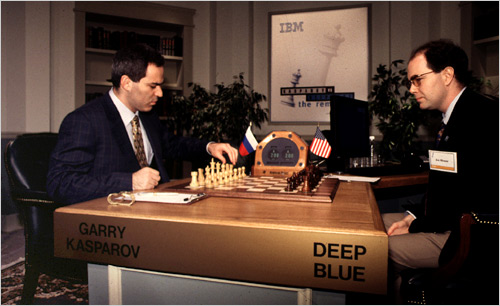
\includegraphics[width=0.60\columnwidth]{images/DeepBlue.png}%
		\caption{Garry Kasparov contre Deep Blue d'IBM}%
	\end{center}
\end{figure}

\newpage
\subsection{Les premières IA pour le jeu vidéo}
Dans les années 1970, les premiers jeux avec des modes 1 joueur apparaissent. Les plus remarquables sont Chasse au Wumpus et Star Trek en 1972 qui utilisaient des Stored Patterns\footnote{Les stored patterns sont des suites d’instructions répétées en boucle par l’agent. Hormis ce qui lui est dit de faire, il ne fera rien d’autre}  pour implémenter les IA des ennemis. L’utilisation des microprocesseurs a permis une augmentation du nombre de mouvement. 

Dans la fin des années 1970 et jusqu’au début des années 1990 : c’est l’âge d’or des jeux d’arcade. Les IA se popularisent. Nombre de jeux (comme Space Invaders en 1978 et Galaxian en 1979) intégraient maintenant une IA plus complexe avec différents niveaux de difficulté et de nombreux modèles de mouvement. 

\begin{itemize}
	\item Pacman (1980) a introduit un pattern IA pour les jeux de labyrinthe, avec des personnalités distinctes pour chaque ennemi.
	\item Karate Champ (1984) a quant à lui introduit le pattern pour les jeux de combat.
	\item First Queen (1988) était un RPG dans lequel des personnages contrôlés par l’IA devaient suivre un leader. Ce type d’IA ayant été amélioré par Dragon Quest IV (1990) avec le system « Tactics » (ajustement des routines utilisées par les IA) puis Secret of Mana (1993).
\end{itemize}

A partir des années 1990, l’émergence de nouveaux genres de jeux vidéo a conduit à l’utilisation d’outils plus sophistiqués tels que les automates finis. Les stratégies en temps réel requéraient la prise en compte de nombreuses contraintes : de nombreux objets, des informations incomplètes, la recherche de chemin, l’économie du nombre de calculs lors de la planification, etc. 

Les premiers jeux rencontraient de nombreux problèmes (Herzog Zwei en 1989 avec une recherche de chemin basée sur un automate fini à trois états, ainsi que Dune 2 en 1992 qui utilisaient de nombreuses « astuces »). 

\newpage
\subsubsection{Une IA évolutive}

Longtemps délaissée au profit des graphismes des jeux vidéo, cette branche constitue maintenant une part importante du travail dans un jeu vidéo. Les joueurs réclament de plus en plus des IA au comportement humain afin d'accroître le sentiment d’immersion. Certains jeux sont réputés pour être des précurseurs en matière d’IA, en voici quelques exemples : 

\begin{itemize}
	\item \textbf{Creatures} (1998) : ce jeu est célèbre pour être le premier à utiliser l’apprentissage automatique lors d’une simulation interactive. A l’aide des réseaux de neurones, les créatures (appelées « Norms ») apprennent divers comportements. Ils peuvent ainsi interagir avec leur environnement. 

	\item \textbf{Halo : Combat Evolved} (2001) : ce jeu utilisait des arbres pour déterminer le comportement des PNJs (« Behavior Tree »), avec beaucoup d’attention portée sur le moindre détail du jeu. Ainsi, la gestion des groupes de PNJs était particulièrement bonne et a joué un rôle de précurseur. 

	\item \textbf{F.E.A.R.} (2005) : l’IA utilise un planificateur (« Planner ») afin de générer des comportements sensibles au contexte, ce fut la première fois dans un jeu grand public. On ressent une grande habileté chez les PNJs. Ils sont en effet capables de trouver une couverture derrière des tables, basculer des étagères, ouvrir des portes, passer à travers les fenêtres, etc. Ce jeu constitue une référence en la matière.  

	\item \textbf{Black \& White} (2001) : le jeu propose au joueur d’incarner une divinité et de guider un peuple. Pour l’aider dans cette tâche, le joueur devra éduquer sa créature, un agent qu’il sera possible de récompenser après une action pour renforcer ce comportement, ou punir, afin de le diminuer. 
\end{itemize}

\newpage
\subsubsection{Une nouvelle perspective pour l’IA}

Machine learning avec du Deep Neural Network

IA with procedural content

\newpage
\section{Les applications possibles prometteuses}

Dans cette section, nous aborderons certaines des techniques les plus utilisées dans les jeux vidéo, ou qui 

\subsection{Le Machine Learning, l’IA qui apprend en même temps que le joueur}

\subsubsection{Les réseaux de neurones}

Un réseau de neurones artificiel (RNA) est un paradigme de traitement de l’information qui est inspiré de la façon par laquelle le système nerveux biologique, telle que le cerveau, traite l’information. L’élément clé de ce paradigme est la structure novatrice utilisée pour le système de traitement de l’information. Il est composé d’une grande quantité d’éléments de traitement grandement interconnectés (neurones), qui, en travaillant à l’unisson résolvent des problèmes spécifiques. Les RNA, comme les humains, apprennent par l’exemple. Un RNA est configuré pour une application particulière, comme la reconnaissance de motifs ou la classification de données, à travers une procédure d’apprentissage. Apprendre, dans le système biologique, implique des ajustements au niveau des connections synaptiques qui existent entre les neurones. C’est également vrai pour les RNA.

La simulation de réseaux de neurones apparaît comme étant un développement récent. Cependant, ce domaine a été établi avant l’avènement des ordinateurs, et a survécu à au moins un revers majeur et à plusieurs époques. Le premier réseau de neurones artificiel fût produit en 1943 par le neurophysiologiste Warren McCulloch et le logicien Walter Pits. Mais la technologie disponible à cette époque n’a pas permis d’en faire grand-chose.

Les réseaux de neurones, avec leur remarquable capacité de déduire un sens à des données compliquées ou imprécises, peuvent être utilisés pour extraire des motifs ou pour détecter des tendances qui sont trop complexes pour être notifiés par des humains ou bien même d’autres techniques informatiques. Un réseau de neurones entraîné peut être assimilé à un « expert » dans la catégorie d’information qu’il analyse. Cet expert peut être utilisé pour fournir des prévisions en lui donnant de nouvelles situations et répondre à des questions du type « Que se passerait-il si … ? ».

D’autres avantages incluent :
\begin{itemize}
	\item L’apprentissage adaptatif : Cette capacité permet d’apprendre comme effectuer des tâches  suivant les données choisies pour l’entrainement or pour l’expérience initiale.
	\item L’auto-organisation : Un RNA peut créer sa propre organisation ou représentation de l’information qu’il reçoit pendant la période d’apprentissage.
	\item Les opérations en temps réel : Les calculs du RNA peuvent être effectués en parallèle, et des équipements spéciaux qui prennent en compte de cette capacité sont en voie de construction.
\end{itemize}

\begin{figure}[!h]%
	\begin{center} 
		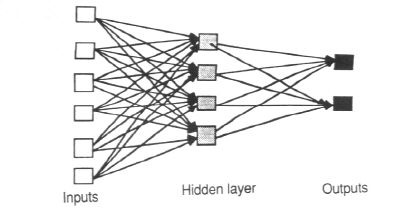
\includegraphics[width=0.60\columnwidth]{images/rna.jpg}%
		\caption{Un simple réseau de neurones}%
	\end{center}
\end{figure}

Le type de réseau de neurones artificiel le plus commun est composé de trois groupes, ou couches, d’unités : une couche d’unités dites « d’entrée » qui est connectée à une couche d’unités « cachées », qui elle-même est connectée à la couche d’unités de « sortie ».

\begin{itemize}
	\item L’activité des unités d’entrée représente l’information brute transmise au réseau.
	\item L’activité des unités cachées est déterminée par celle des unités d’entrée et des connections pondérées entre les unités d’entrée et celles cachées.
	\item Le comportement des unités de sortie dépend de l’activité des unités cachées et des liaisons pondérées entre les unités cachées et celles de sortie.
\end{itemize}

Ce type simpliste de réseau de neurones est intéressant car les unités cachées sont libres de construire leur propre représentation de leurs entrées. Ces poids entre les unités cachées et les unités d’entrée déterminent la valeur d’activité d’une unité cachée, et donc en modifiant ces valeurs, une unité cachée peut choisir ce qu’elle représente.

On peut distinguer les architectures monocouche ou multicouche. Les organisations monocouches, dans lesquelles toutes les unités sont connectées aux autres, constituent le cas le plus général et un plus grand potentiel de puissance de calcul que les organisations multicouches structurées par hiérarchie. Dans les réseaux multicouches, les unités sont numérotées par couche au lieu de suivre une numérotation globale.

Il existe plusieurs stratégies d’apprentissage pour un réseau de neurones artificiel :
\begin{itemize}
	\item \textbf{L’apprentissage supervisé} : Cette stratégie implique un professeur plus intelligent que le réseau lui-même, qui servira de superviseur pour l’apprentissage du réseau de neurones. Par exemple, dans le cas de la reconnaissance faciale, le professeur connaît déjà les noms des personnes qu’il montre au réseau de neurones. Il peut ainsi comparer les réponses données par le réseau et déterminer si des ajustements sont à faire.
	
	\item \textbf{L’apprentissage non supervisé} : Cette technique est requise lorsqu’il n’existe pas d’exemples d’ensembles de données possédant des réponses connues. Prenons par exemple la recherche d’un motif caché dans un ensemble de données. Une application de cela est le « clustering », c’est-à-dire la division en groupes d’un ensemble d’éléments suivant une disposition inconnue.
		
	\item \textbf{L’apprentissage par renforcement} : Cette stratégie est basée sur l’observation. Prenons par exemple un petit robot circulant à travers un labyrinthe. Si le robot tourne à gauche, il obtient une récompense, s’il tourne à droite il hérite d’un malus. On peut supposer que le robot apprendra avec le temps à tourner à gauche. Son réseau de neurones prend une décision avec une valeur d’entrée (tourner à gauche ou à droite) et observe son environnement (récompense ou malus). Si l’observation est négative, le réseau peut ajuster les valeurs des poids entre les unités du réseau afin d’effectuer un choix différent la prochaine fois. L’apprentissage par renforcement est une technique commune dans le domaine de la robotique.
	Cette capacité qu’a le réseau de neurones à apprendre, à faire des ajustements sur sa propre structure à travers le temps, est ce qui le rend si utile dans le domaine de l’intelligence artificielle.
\end{itemize}

Avantages

Inconvénients

\newpage
\subsubsection{Les arbres de décision avec l’apprentissage par renforcement}

Avantages

Inconvénients

\newpage
\subsection{Dynamic Game Difficulty Balancing, l’IA qui s’adapte au niveau du joueur}

Beaucoup d’exemples assez simple (on augmente automatiquement le niveau/nombre des ennemis, etc si on trouve que le joueur s’en sort bien, et inversement) 

Les fameux items de Mario Kart (plus t’es loin, meilleurs sont tes objets)

Le meilleur exemple pour ce type d’IA se trouve du côté de Valve, et plus précisément dans leur FPS de survival horror, Left 4 Dead. Dans celui-ci, là on explique brièvement le jeu, on sait jamais. Et, contrairement à beaucoup de jeux dans lesquels la difficulté augmente de façon constante, ici un “AI Director” analyse constamment les performances individuelles et collectives des joueurs pour construire une expérience adaptée à tous.

\begin{figure}[!h]%
	\begin{center} 
		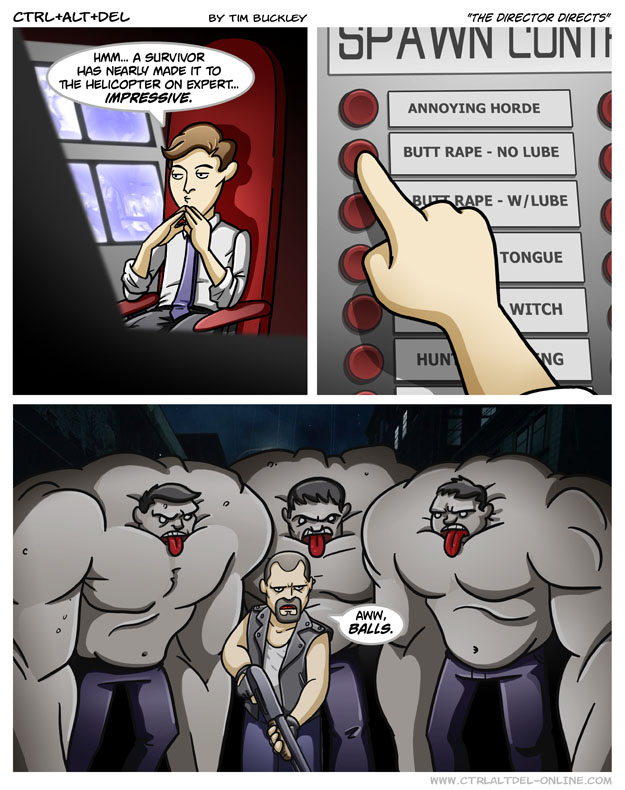
\includegraphics[width=0.60\columnwidth]{images/aiDirector.png}%
		\caption{The Director Directs, de Tim Buckley}%
	\end{center}
\end{figure}

\newpage
\subsection{Des jeux par les IA, pour les IA}

Bientôt, il n’y aura plus du tout besoin d’humains dans la boucle de création et consommation de jeu.

En effet, la prochaine IA dont nous allons parler est une IA capable d’apprendre à joueur à des jeux, tandis que la suivante, très jeune, est capable de développer des jeux (simples) complets.

\subsubsection{General Game Playing, l'IA qui apprend à jouer}

C’est un domaine qui a gagné en popularité ces dernières années, notamment grâce à une IA qui a gagné le prix du public de la compétition annuelle organisée par l’AAAI (Association for the Advancement of Articifial Intelligence).

Cette IA est capable d’apprendre à jouer à un niveau de Mario Bros (un jeu de plateforme 2D) et de s’adapter aux différents niveaux qui le composent.

\newpage
\subsubsection{Angelina, l’IA qui développe des jeux}

Angelina est une IA qui, à partir d’une description en langage naturel, peut générer des jeux de plateforme 2D, avec une ambiance, des graphismes et un gameplay qui respectent (dans une certaine mesure) la description fournie.

C’est un sujet de recherche développé par Michael Cook, un chercheur britannique à l’université de Falmouth.

\begin{figure}[!h]%
	\begin{center} 
		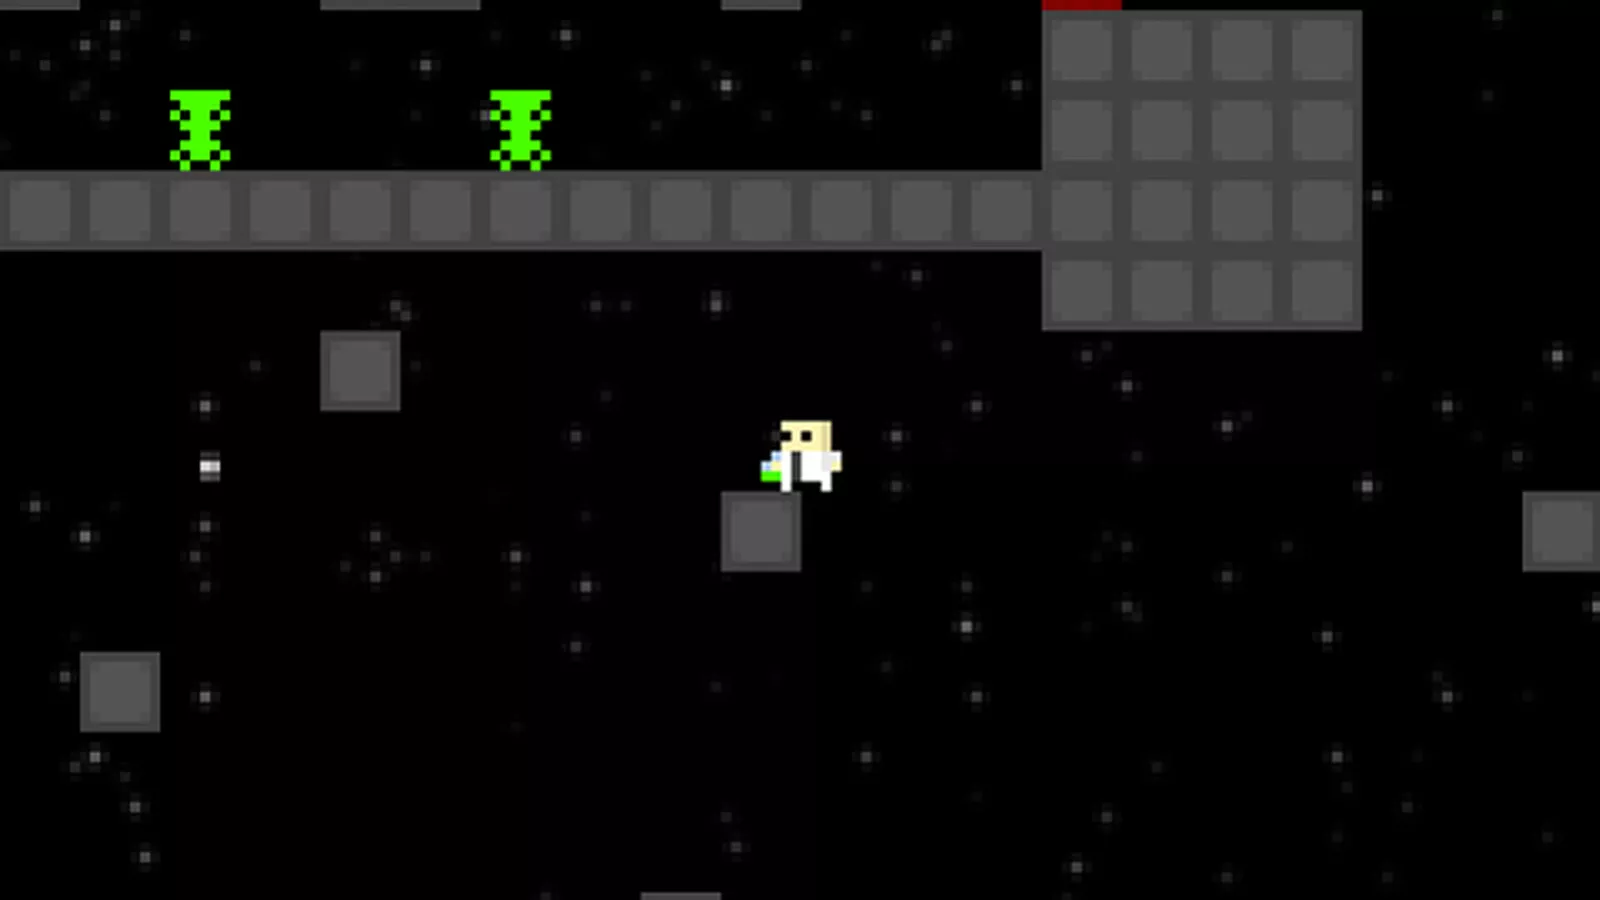
\includegraphics[width=0.60\columnwidth]{images/angelina.png}%
		\caption{Exemple de jeu produit par Angelina}%
	\end{center}
\end{figure}

Pour arriver à ce résultat, elle analyse la description, <<<DESCRIPTION>>>

%------------------------------------------------

\newpage
\section{De l’importance de l’IA pour l’immersion du joueur}

Dans cette partie, nous parlerons de l’intelligence artificielle qui n’est pas flagrante, mais qui rend, inconsciemment pour le joueur, l'expérience de jeu plus réaliste et immersive. Cette intelligence artificielle est principalement importante dans les jeux à un seul joueur, dans lesquels l’immersion est bien plus importante que dans les jeux multi-joueurs, dans lesquels il est dur de maintenir le joueur dans un univers fictif à cause de la présence d’autres joueurs dont le comportement est difficilement contrôlable et peut être perturbateur.

\begin{figure}[!h]%
	\begin{center} 
		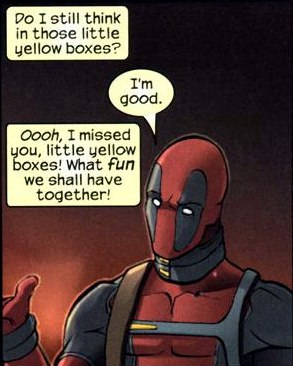
\includegraphics[width=0.60\columnwidth]{images/deadpool.png}%
		\caption{Deadpool, personnage de l’univers Marvel connu pour ne pas beaucoup respecter le 4ème mur}%
	\end{center}
\end{figure}

\newpage

\subsection{Suspension consentie de l'incrédulité, solipsisme et vallée dérangeante}

\begin{wrapfigure}{r}{0.4\textwidth}
	\begin{center}
		
\includegraphics[width=0.38\textwidth]{images/repeat1.png}
	\end{center}
	\caption{Why RPG NPCs Always Repeat Themselves, de Dorkly}
\end{wrapfigure}

Lorsqu’un PNJ répète sans cesse le même dialogue au joueur, celui-ci est ramené à la réalité. Quand un PNJ rencontre un problème de recherche de chemin (lorsqu’un PNJ fonce obstinément dans un mur) ou n’arrive pas à se déplacer d’un point à un autre, le joueur est ramené brutalement à la réalité. 

Toutes ces actions, souvent sans le vouloir, cassent le quatrième mur, et mettent fin à ce que l’on appelle la Suspension Consentie de l’Incrédulité (aussi connue sous le nom de Suspension of disbelief en anglais). Il s’agit d’une sorte de contrat que le joueur signe avec l’œuvre de fiction (que ce soit un jeu, un film, un livre), dans lequel le joueur accepte de mettre de côté son scepticisme le temps de la consultation de l’œuvre en question. 

\begin{figure}[!h]%
	\begin{center} 
		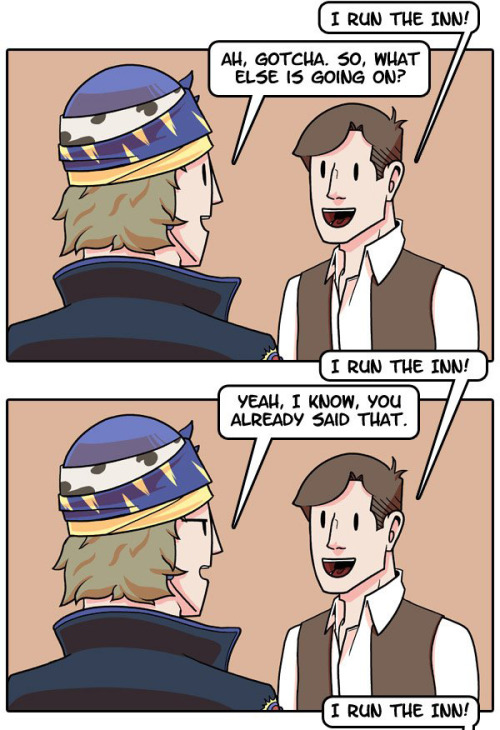
\includegraphics[width=0.42\columnwidth]{images/repeat2.png}%
		\caption{Why RPG NPCs Always Repeat Themselves, de Dorkly}%
	\end{center}
\end{figure}

Il peut ainsi s’immerger dans un univers avec des éléments imaginaires, pour peu que ceux-ci restent crédibles, et que les règles qui régissent l’œuvre restent constantes.
Lorsque ce contrat est rompu (par définition, il ne peut être rompu que par l’œuvre de fiction), il est difficile de faire replonger un joueur dans l’univers du jeu, avec lequel il restera toujours un peu distant, et cela renforce le solipsisme du joueur.

\newpage
\subsubsection{Solipsisme}

Le solipsisme (du latin \textbf{\textit{solus}}, « seul » et \textbf{\textit{ipse}}, « soi-même ») est une attitude selon laquelle, la seule certitude absolue pour le sujet pensant, est que lui-même existe. Cette attitude est répandue dans la société, et il est tout à fait normal de l’avoir ressenti de façon passagère.

Mais c'est dans les jeux vidéo (principalement ceux à un seul joueur) qu'elle est le plus présente, et qu’on essaie le plus de la faire disparaître. En effet, le but d’un jeu narratif est d’immerger le joueur, et un très bon moyen pour cela est de lui faire oublier qu’il est la seule personne effectivement douée de conscience.

\begin{figure}[!h]%
	\begin{center} 
		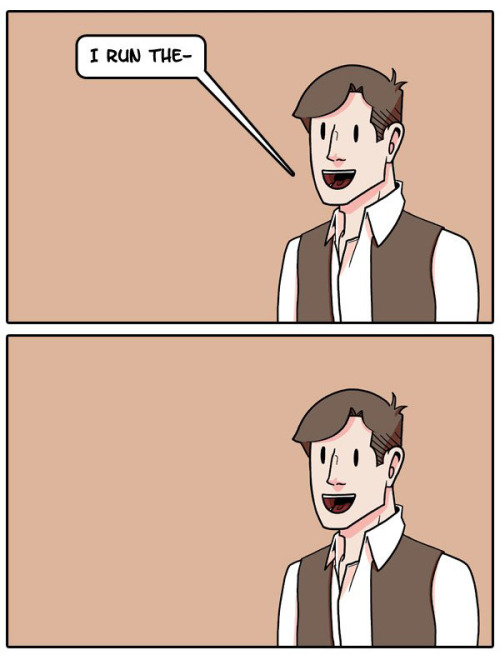
\includegraphics[width=0.60\columnwidth]{images/repeat3.png}%
		\caption{Why RPG NPCs Always Repeat Themselves, de Dorkly}%
	\end{center}
\end{figure}

Evoluer dans un monde photoréaliste et crédible est un bon moyen de garder le joueur immergé. Toutefois, rares sont les jeux sans PNJ, il faut donc s’assurer qu’eux aussi ne cassent pas cette immersion. Pour cela, les doter de réactions naturelles est la manière la plus efficace pour arriver à ce résultat.

Ainsi, de de plus en plus de développeurs de MMORPG (Jeu de Rôle Massivement Multijoueur) décident de donner plus de profondeur aux PNJ (amicaux comme ennemis).

C’est le cas notamment dans EverQuest Next, dans lequel chaque PNJ se voit attribuer certains traits de caractère, ce qui affecte la façon dont il interagit avec les joueurs, ainsi qu’avec les autres PNJ. 

De plus, toujours dans EverQuest Next, les monstres ne sont pas regroupés en « camps de monstres », dans lesquels ils ne font qu’attendre, immobiles et apathiques, qu’un joueur vienne les sortir de leur léthargie, comme c’est le cas dans beaucoup de MMORPG actuels. 

Par exemple, un monstre pourra former un groupe avec d’autres monstres et tendre des embuscades sur une route, et soit se faire chasser par des joueurs, soit partir vers d’autres horizons s’ils jugent que cette zone n’est pas assez fructueuse.

Toutefois, si le réalisme du comportement des PNJ dépasse un certain point, mais n’arrive pas à la hauteur des attentes du joueur, celui-ci peut être confronté à la vallée dérangeante (plus connue sous son nom anglais d’Uncanny Valley).

\begin{figure}[!h]%
	\begin{center} 
		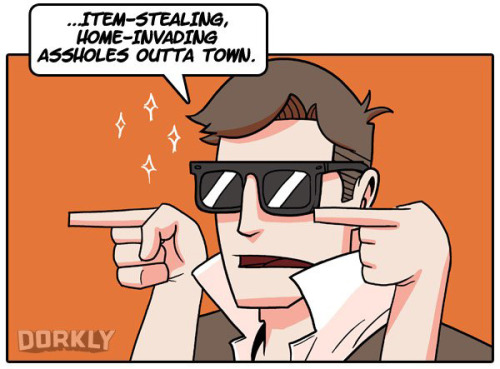
\includegraphics[width=0.60\columnwidth]{images/repeat4.png}%
		\caption{Why RPG NPCs Always Repeat Themselves, de Dorkly}%
	\end{center}
\end{figure}

\newpage
\subsubsection{Vallée dérangeante}

La vallée dérangeante est une théorie selon laquelle plus une créature à forme humaine ressemble à un être humain, plus on remarque ses imperfections, même minimes, et plus elles nous dérangent. Cette théorie a été publié en 1970 par le roboticien Japonais Masahiro Mori, dans le cadre de ses recherches sur les réponses émotionnelles des robots.

\begin{figure}[!h]%
	\begin{center} 
		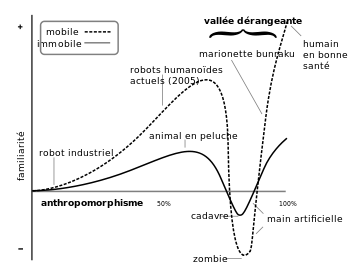
\includegraphics[width=0.60\columnwidth]{images/uncannyValley.png}%
		\caption{Réaction émotionnelle supposée de sujets humains à l'anthropomorphisme (Wikipédia) }%
	\end{center}
\end{figure}

Dans les jeux vidéo, c’est le plus souvent dû au physique (proportions du corps) et à l’animation (principalement du visage) des personnages humanoïdes, qui se rapprochent de plus en plus de la perfection, et qui donc, à la moindre imperfection, nous paraissent monstrueux.

\begin{figure}[!h]%
	\begin{center} 
		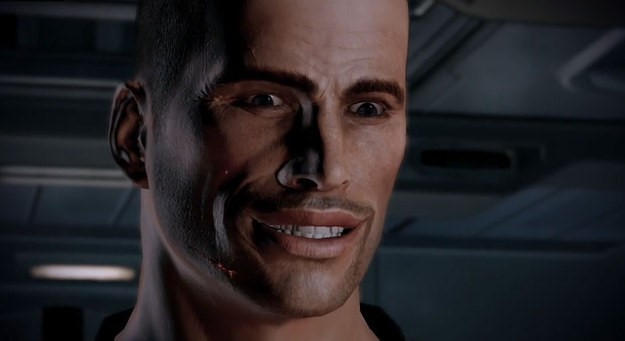
\includegraphics[width=0.60\columnwidth]{images/shepard.jpg}%
		\caption{Commandant Shepard et son sourire dérangeant, Mass Effect 3, BioWare}%
	\end{center}
\end{figure}

Toutefois, le comportement des PNJ joue également un rôle très important. Le personnage de Natalya, personnage secondaire de GoldenEye 007 (Nintendo 64, 1997) notamment, est devenu célèbre pour ses piètres capacités intellectuelles. En effet, plusieurs missions le long du jeu requièrent de l’escorter d’un endroit à un autre en la gardant en vie. Hors, en présence d’ennemis, Natalya n’hésitera pas à se jeter fièrement dans la bataille, bien qu’elle ne puisse ni attaquer ni se défendre, ce qui dans la plupart des cas la mènera à sa mort, et donc à l’échec de la mission.

\begin{figure}[!h]%
	\begin{center} 
		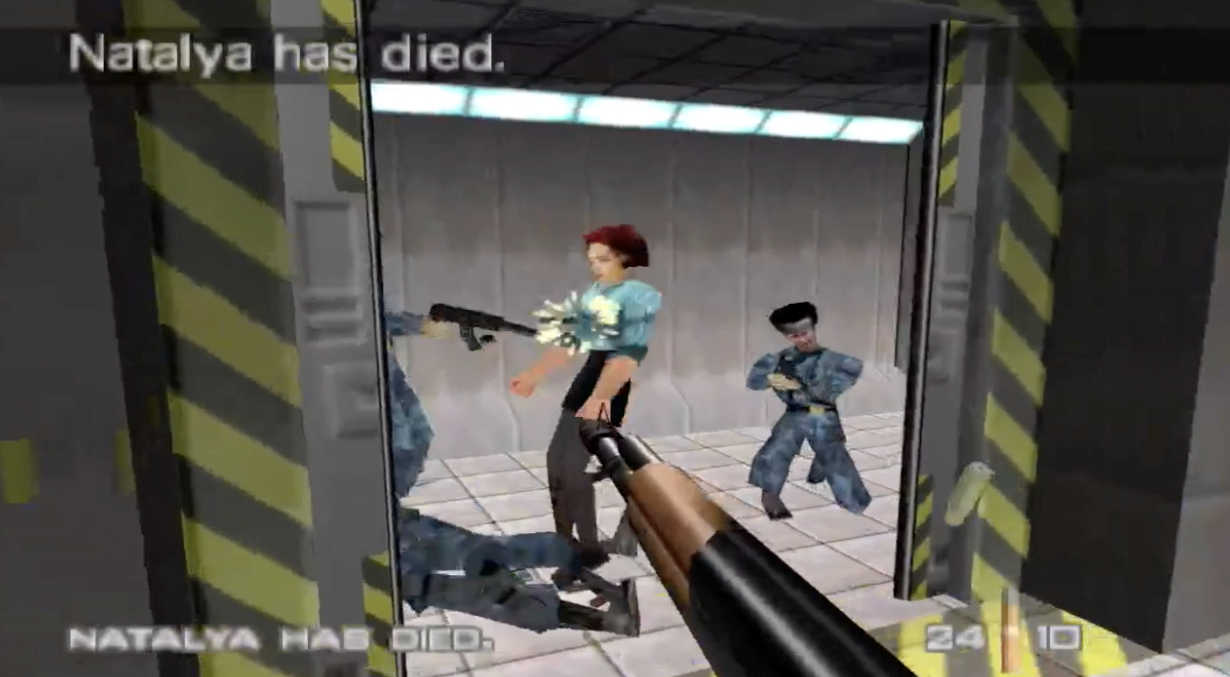
\includegraphics[width=0.60\columnwidth]{images/natalya.png}%
		\caption{Natalya, regrettant sa décision de se jeter au milieu de PNJ hostiles}%
	\end{center}
\end{figure}

Lorsque ce n’est pas un être humanoïde qu’il voit agir de façon si incohérente, le joueur peut imaginer des causes, ou même ne pas vraiment comprendre mais se dire qu’il lui manque les clés pour comprendre le comportement du PNJ si le joueur ne peut pas s’identifier à lui. 

Mais lorsqu’un humain voit un autre être qui lui ressemble, il ne peut s’empêcher d’essayer de se mettre à la place de l’autre et de le comprendre. Ainsi, pour un joueur, être témoin d’un comportement étrange et inexplicable d’un PNJ a forme humanoïde est une expérience parfois drôle, mais souvent désagréable, et qui nuit toujours à l’immersion.

\newpage
\subsection{Entre la sérendipité et l'apophénie}

De par son côté de plus en plus évolutif et complexe, il est parfois difficile de prévoir tous les résultats possibles d’une interaction du joueur avec l’IA, ce qui donne parfois lieu à une sorte de gameplay émergent, avec des PNJ au comportement imprévisible, même pour les créateurs.

Si dans les jeux, cet aspect peut presque passer inaperçu, comme dans Fable et n'est pas très présent, certains programmes reposent essentiellement sur ce principe, comme le chatbot Evie (Evie n'est pas un jeu vidéo au sens classique du terme, mais cela reste un programme ludique avec lequel le joueur peut interagir).

\newpage
\subsubsection{Fable, un monde plus vivant qu'il n'y paraît}

Fable est un jeu sorti en 2004, et innovant pour son époque, de par la liberté qu’il laisse au joueur. En effet, le joueur peut se marier, divorcer, boire, jouer aux cartes, acheter, louer et revendre une ou plusieurs maisons, se tourner vers les forces obscures ou le bien, massacrer des innocents, des gardes ou des bandits, entre autres activités diverses et variées.

Ce qui suit est une anecdote tirée du blog d’un des développeurs, traduite, adaptée et commentée.
Les développeurs se sont également imposés deux règles qu’ils jugeaient vitales que le jeu suive, sans quoi il ne respecterait pas leur vision :

\begin{itemize}
	\item Le monde dans lequel le joueur évolue, ainsi que tous ses occupants doivent réagir de manière appropriée aux actions du joueur.
	\item Le personnage principal doit exprimer visuellement ce qu’il ressent.
\end{itemize}
	
\textbf{Un monde simulé}

Pour rendre le monde plus intéressant, les développeurs ont donné à chaque PNJ leurs propres traits de caractères, comme dans EverQuest Next (PC, en développement).

\begin{wrapfigure}{r}{0.4\textwidth}
	\begin{center}
		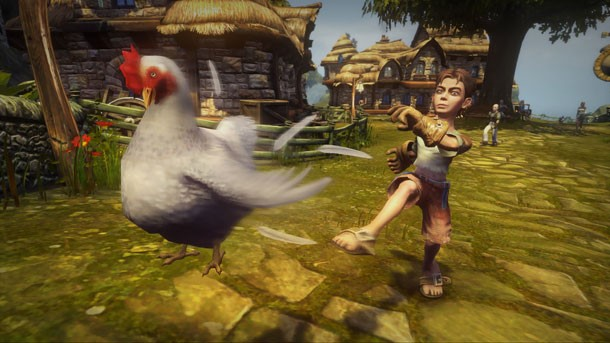
\includegraphics[width=0.38\textwidth]{images/chicken.jpg}
	\end{center}
	\caption{Enfant tourmentant une poule dans Fable}
\end{wrapfigure}

Ils ont également remarqué que les joueurs étaient particulièrement sensibles aux émotions des enfants. Ils ont donc décidé de rendre le comportement des enfants très varié. Ainsi, certains sont de véritables petites pestes (comme certains le sont dans la réalité), et poursuivent et tourmentent les poules, tandis que d’autres vont à l’école bien en rangs, et rentrent gentiment à la maison à l’heure pour le goûter (comme certains le font dans la réalité).

Et, peut-être le plus important, les enfants fixeront avec intensité ce qu’ils trouvent intriguant.

\textbf{Un héros expressif}

Plutôt que d’afficher plein de caractéristiques comme dans un RPG classique, les développeurs ont trouvé plus intéressant de montrer par des mouvements et des expressions que le personnage réagit au monde qui l’entoure (plutôt que de rester planter là, sans émotions apparentes).

\textbf{Un héros expressif dans un monde simulé}

Quand on mélange les deux, voici ce que cela peut donner :

Imaginez-vous la scène, une radieuse journée à Bowerstone (une ville du jeu). Les papillons papillonnent, le parfum des tulipes vous est porté par une brise. Au loin, on entend des enfants jouant et rigolant dans une cour de récréation, réticent à retourner en classe, malgré le son de cloche qui signifie la fin de la pause.

Le cours a repris, après quelques remontrances de l’institutrice. Un des enfants, trouvant le cours assommant, regarde par la fenêtre en soupirant.

L’homme s’infiltre silencieusement dans l’école. L’institutrice lui tourne le dos. Elle ne se doute de rien.

Un par un, les enfants se mettent à fixer quelque chose derrière l’institutrice. La classe devient silencieuse. Finalement, l’institutrice entend un bruit derrière elle, se retourne et …

… tombe nez à nez avec un homme en caleçon, planté au milieu de sa salle de classe, souriant à pleines dents. Soudain, souriant de plus belle, il fait un doigt d’honneur. Tout le monde hurle …

\textbf{Ce qu'il s'est vraiment passé}
\begin{itemize}
	\item Le personnage sourit car il se sent sécurité.
	\item Les enfants fixent ce qui leur semble intéressant (ici, le personnage, qui est une nouveauté pour eux).
	\item Le doigt d’honneur est considéré comme un acte d’agression, d’où les cris.
\end{itemize}	

On pourrait ici presque parler de « comportement émergent » (en parallèle au gameplay émergent, dans lequel les joueurs trouvent de nouvelles façons de jouer que les développeurs n’avaient pas prévu) car en partant de règles simples, on arrive à une situation complexe et crédible.

C’est un bon exemple d’apophénie (fait de donner un sens particulier à des évènements banals), car le joueur interprète les réactions des PNJ différemment de ce que les développeurs avaient probablement en tête lors de la réalisation du jeu. 

\newpage
\subsubsection{De ELIZA à Evie}

Un agent conversationnel (ou chatbot en anglais), est un logiciel autonome qui a pour fonction de dialoguer avec l’utilisateur. Pour cela, la phrase entrée par l’utilisateur est traduite en un langage intermédiaire pour permettre à l’agent de l’analyser, qui va ensuite générer une réponse plus ou moins approprié.

ELIZA, créé en 1966, par Joseph Weizenbaum, MIT, fut le premier agent conversationnel développé. Son comportement était très simple et scripté (elle répondait aux questions en demandant pourquoi cette question, si elle détectait le mot « ordinateur », elle demandait si la question lui avait posée parce qu’elle est une machine), et laissait donc peu de place à une vraie conversation.


\begin{figure}[!h]%
	\begin{center} 
		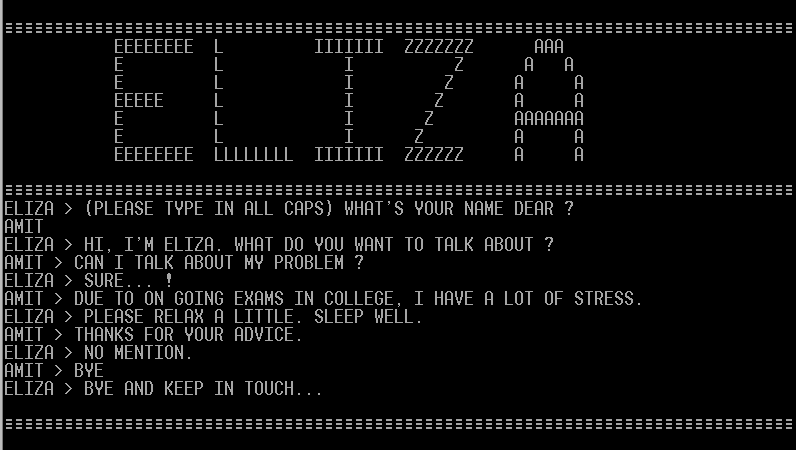
\includegraphics[width=0.60\columnwidth]{images/eliza.png}%
		\caption{ELIZA, premier chatbot}%
	\end{center}
\end{figure}

En 1997, Rollo Carpenter, un informaticien britannique, crée Jabberwacky. C’est lui aussi un agent conversationnel, mais au lieu d’avoir un comportement scripté, celui-ci est capable d’apprendre. En effet, il stocke dans une base de données toutes les conversations des utilisateurs, et s’en sert pour choisir une réponse à la question posée par l’utilisateur.

Ce n’est que onze ans plus tard, en 2008 que Rollo Carpenter met en ligne Cleverbot, descendant spirituel de Jabberwacky. Celui-ci dispose également d’une base de données des conversations avec les utilisateurs parmi lesquelles il va chercher la réponse la plus appropriée, mais a également une notion de contexte, grâce à un système de mémoire à court terme, qui donne un poids plus important aux conversations récentes.

\newpage
\begin{figure}[!h]%
	\begin{center} 
		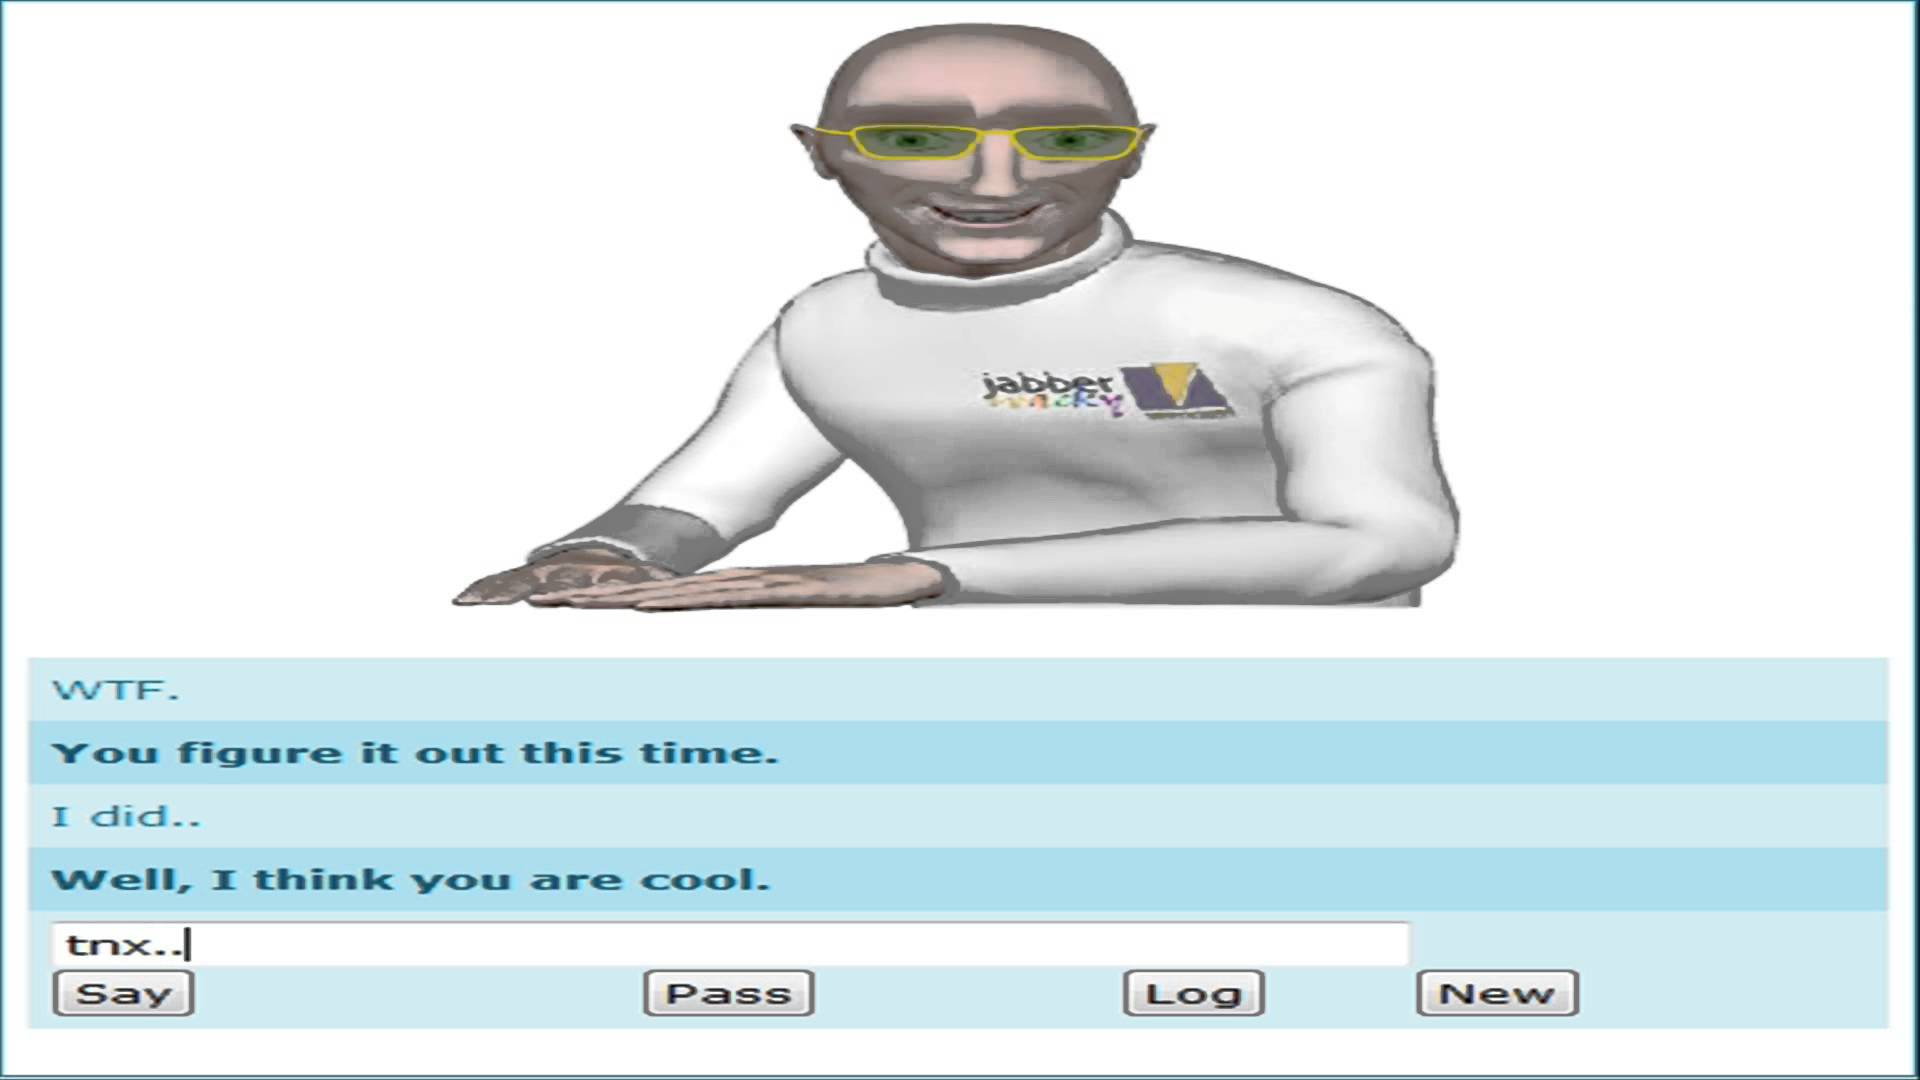
\includegraphics[width=0.60\columnwidth]{images/jabberwacky.jpg}%
		\caption{Jabberwacky, en pleine discussion}%
	\end{center}
\end{figure}

C'est également à ce moment que Existor voit le jour, fondé par Rollo Carpenter, entreprise qui se donne pour objectif de développer des technologies pour arriver à un niveau de conversation humain.

Ainsi, c’est en 2015 que Evie (Electronic Virtual Interactive Entity), la petite sœur de Cleverbot, voit le jour. Devant la quantité de données que les différents chatbot de Existor récoltent chaque jour (5.5 millions de conversations par jour), et le nombre impressionnant de 1.5 milliards de conversations enregistrées, les développeurs de Existor ont commencé à utiliser des techniques de Machine Learning. 

\begin{figure}[!h]%
	\begin{center} 
		
\includegraphics[width=0.60\columnwidth]{images/evie.png}%
		\caption{Evie}%
	\end{center}
\end{figure}

Dans un premier temps, ils s’en sont servi pour chercher des motifs récurrents dans les phrases, puis, à l’aide de RNNLMs (Recurrent Neural Network Language Models), ils ont pu estimer les probabilités que tels ou tels mots se suivent, afin de former une phrase plus naturelle.

Ainsi, même si les réponses de Evie sont de plus naturelles, le joueur ne sait jamais trop jusqu'où une conversation avec elle peut aller. Comme dans une discussion naturelle, le sujet change au fur et à mesure de la conversation, parfois de manière brusque quand Evie ne comprend pas bien la phrase du joueur, et le joueur peut très vite se retrouver dans une situation dans laquelle Evie l'insulte, ou en train de se battre pour avoir le dernier mot :

\begin{itemize}
	\item Evie : Oui
	\item Joueur : Non
	\item Evie : Oui
	\item Joueur : Non
	\item etc ...
\end{itemize}

%------------------------------------------------

\newpage
\section{Apports du mémoire}
Lors de nos recherches pour écrire ce mémoire, nous avons non seulement approfondi énormément nos connaissances sur beaucoup de sujets qui touchent à l'intelligence artificielle, notamment le machine learning, mais nous avons également découvert plusieurs applications dont nous n'avions aucune idée de l'existence, comme Angelina, l'IA qui développe des jeux.

Cependant, il s'agit d'un sujet tellement vaste que n'avons fait qu'en gratter la surface.

%------------------------------------------------

\newpage
\section{Conclusion}



%----------------------------------------------------------------------------------------
%	BIBLIOGRAPHY
%----------------------------------------------------------------------------------------
\newpage
\bibliographystyle{unsrt}
\bibliography{References}

%----------------------------------------------------------------------------------------

\end{document}
